\begin{problema}
\mbox{}
    \begin{enumerate}
        \item[(i)] 
            Ejecute y explique la funci\'on del siguiente c\'odigo en Octave. Comente qu\'e 
            teoremas del curso (y del curso de probabilidad) son importantes para interpretar 
            la figura.
            \tiny
            \texttt
            {
                \lstinputlisting[caption=]{tarea3/problema3_4/polya2.R}
            }
            \normalsize
            (Conmigo se negó a brincar de linea. Tuve que hacerlo diminuto para que apareciera el código completo.)\par\null
        
        \item[(ii)]
            Ejecute y explique la funci\'on del siguiente c\'odigo en Octave. 
            Incluya una gr\'afica en la que la longitud de la variable k sea mayor a 1000. 
            (Puede modificar el programa...) En la gr\'afica observara un esbozo de la 
            trayectoria de un proceso de ramificaci\'on continuo (en una escala distinta...).
            \texttt{
                \lstinputlisting[caption=]{tarea3/problema3_4/binaryGW.R}
            }
    \end{enumerate}
\end{problema}

\afterstatement\par\null

\begin{center}
    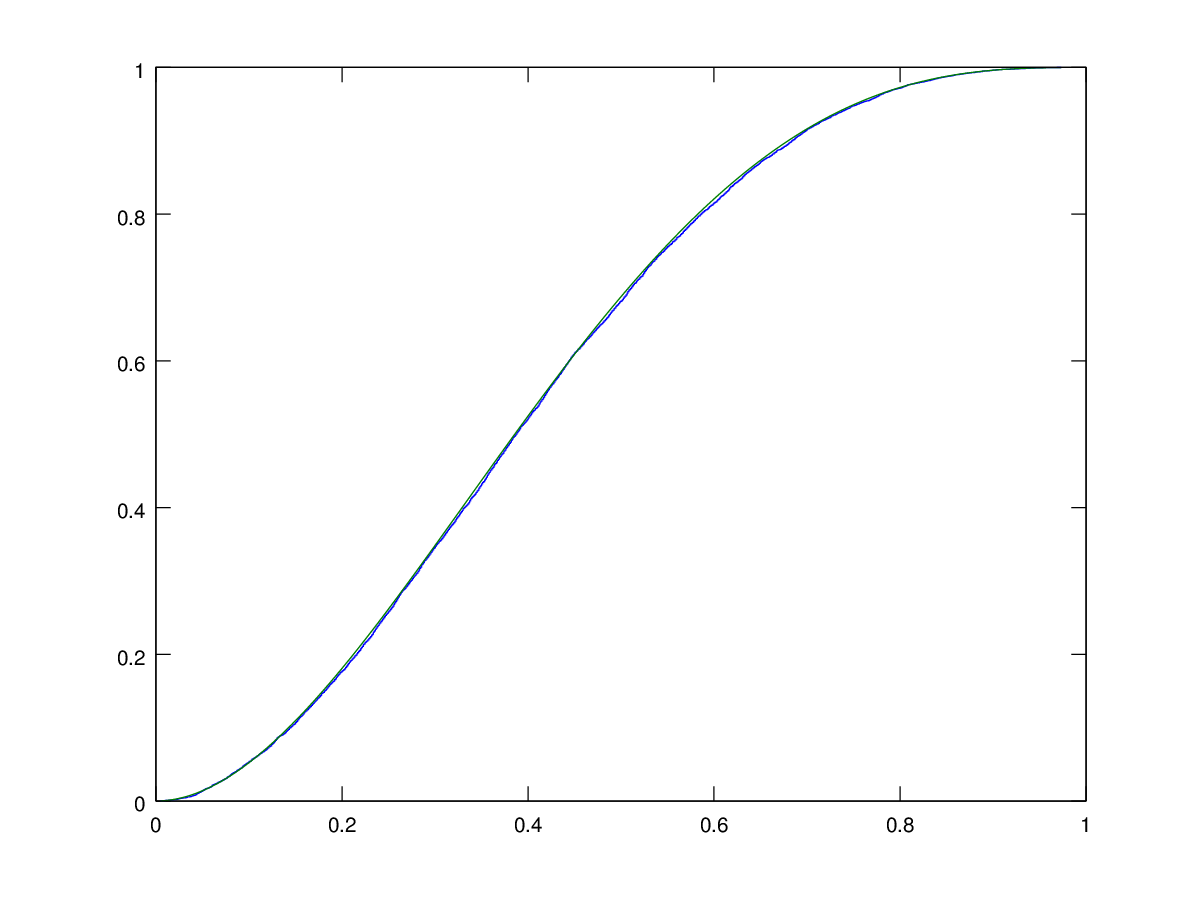
\includegraphics[width=8cm]{tarea3/problema3_4/poylaBeta.PNG}\par\null
    	Gráfica del histagrama de los radios ``finales'' de muchas iteraciones del proceso 
	de urnas de Poyla.
\end{center}

\begin{center}
    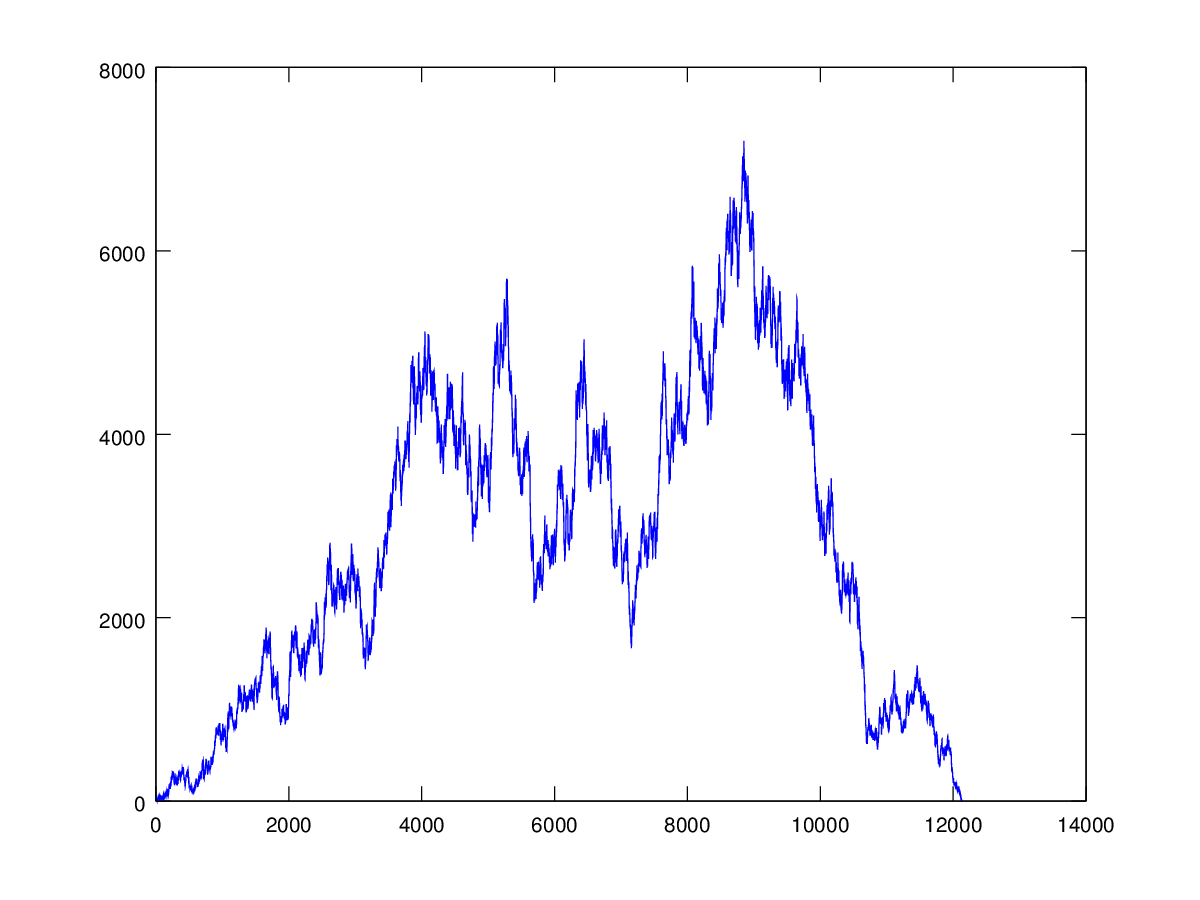
\includegraphics[width=8cm]{tarea3/problema3_4/galtonWatson.PNG}
    
	Gráfica de una ejecución del proceso de extinción de Galton-Watson 
	Parámetros: 10 individuos
	La probabilidad de que un individuo tenga $2$ hijos es $\frac{1}{2}$
	La probabilidad de que un individuo tenga $0$ hijos es $\frac{1}{2}$.
\end{center}